%!TEX root = ../main.tex
\chapter{MARCO TEÓRICO}
\label{ch2:MarcoTeorico}

\section{Imágenes}
Importar imágenes con citas (Fig. \ref{fig:SP}).
\begin{figure}
	\centering{\includegraphics[width=.5\textwidth]{rueda}}
	\caption{Rueda Omnidireccional \protect\cite{itam-gary} }
	\label{fig:SP}
\end{figure}

Tambien se pueden usar imágenes eps y ponerlas en página completa giradas.

\begin{sidewaysfigure}
	\centering
		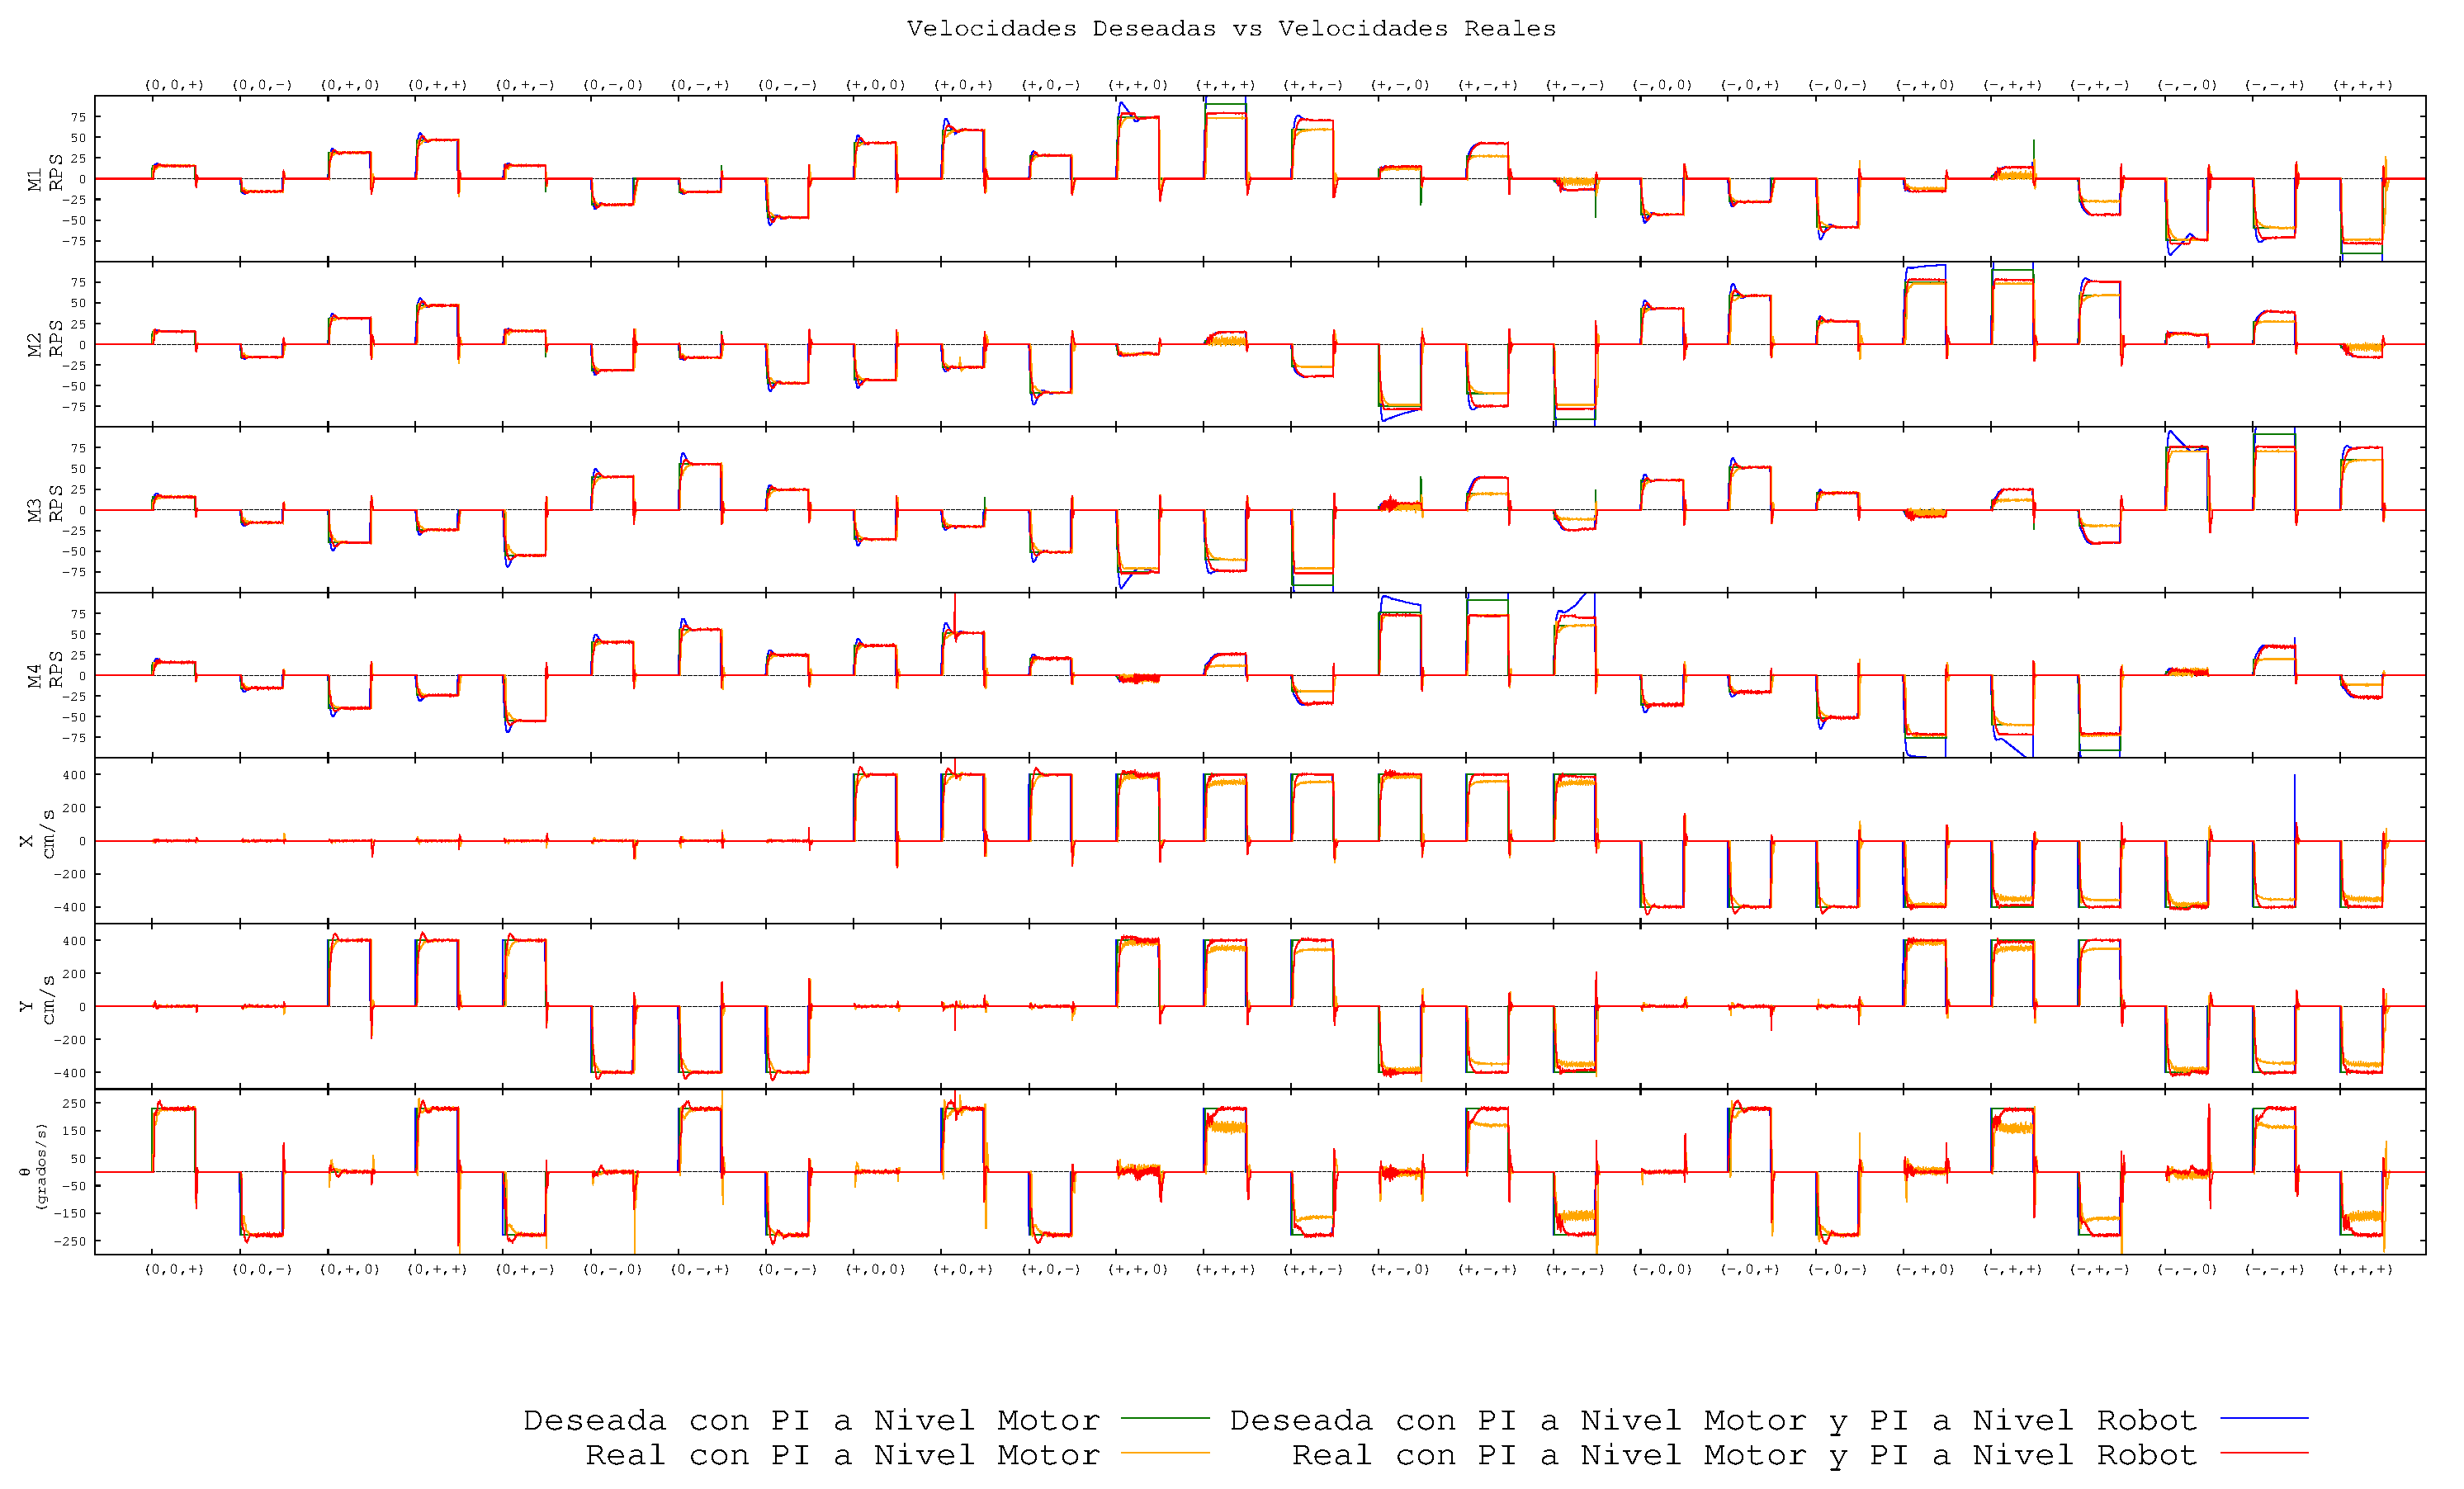
\includegraphics[width=\textwidth,height=0.9\textheight]{Figures/160517-vels-motVSmotrob_slide.eps}
	\caption{Velocidades Deseadas vs Velocidades Reales}
	\label{fig:vels_real_vs_des_mot}
\end{sidewaysfigure}



\section{Acrónimos}
En el archivo auxiliar ``Aux\_files/Glossary.tex'' se definen los términos del glosario.
Es útil usar acrónimos: \gls{ITAM}. Si se usa por segunda vez ya no se expande: \gls{ITAM}. 

\section{Glosario}
Para usar un término del glosario: \gls{Wi-Fi}.

\section{Citas}
En el archivo auxiliar ``Aux\_files/FuentesConsultadas.bib'' se define la bibliografía. Se puede usar como: \cite{turing2009computing}.

{\selectlanguage{english} \blindtext \blindtext \Blindtext}


% \label{robocup-ssl}






